% Chapter Template

\chapter{Performance Analysis and Optimisation}

\label{Chapter6}

\lhead{Chapter 6. \emph{Performance Analysis and Optimisation}}

\section{Performance Analysis using Intel VTune Profiler}
\subsection{Baseline Performance analysis}
\begin{figure}[htbp]
% \begin{figure}[]
    \centering
    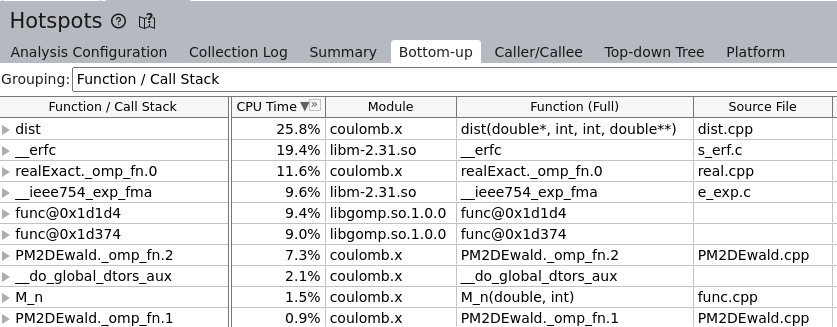
\includegraphics[width = \linewidth]{images/VTuneInitialHotspot.png}
    \caption{Hotspot analysis of the baseline Ewald summation implementation, as reported by Intel VTune Profiler. A significant portion of total CPU time is concentrated in the \textit{dist} function (25.8\%), the standard math library's \textit{\_\_erfc} function (19.4\%).}
    \label{fig:result1}
\end{figure}
\begin{figure}[h]
    \centering
    \begin{minipage}{0.5\textwidth}
        \fbox{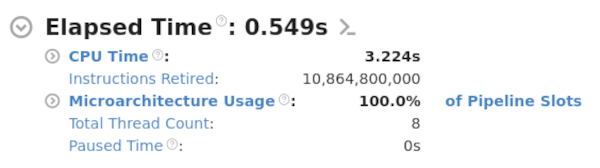
\includegraphics[width=\linewidth]{images/VTuneInitialTime.png}}
    \end{minipage}%
    \begin{minipage}{0.4\textwidth}
        \caption{This is the caption placed on the right side of the image.}
    \end{minipage}
\end{figure}
\subsection{Polynomial Interpolation of Error Function}
During performance profiling using Intel VTune Profiler, it was observed that a significant portion of the program’s execution time was consumed by calls to the \verb|std::erfc| function. This function, part of the C++ Standard Library (\verb|<cmath>| header), computes the complementary error function. These calls' high frequency and computational cost were identified as a key performance bottleneck within the application.
\[
erf(x) = 1 - (a_1 t + a_2 t^2 + a_3 t^3 + a_4 t^4 + a_5 t^5) e^{-x^2} + \epsilon(x),
\]
\[
t = \frac{1}{1 + px}, \quad |\epsilon(x)| \leq 1.5 \times 10^{-7},
\]
\[
p = 0.3275911, \\
a_1 = 0.254829592, \\
a_2 = -0.284496736,
\]
\[
a_3 = 1.421413741, \\
a_4 = -1.453152027, \\
a_5 = 1.061405429.
\]
\subsection{Performance of Optimised Implementation}
\begin{figure}[htbp]
% \begin{figure}[]
    \centering
    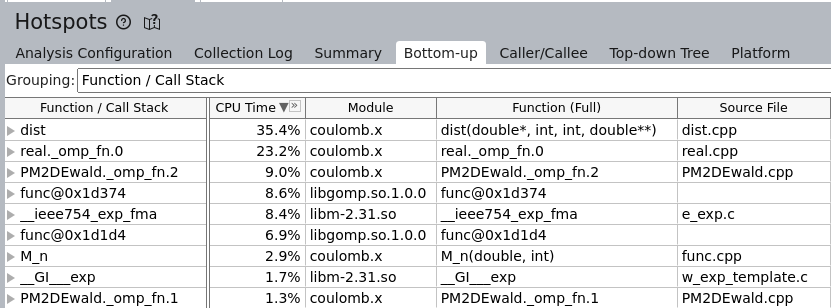
\includegraphics[width = \linewidth]{images/VTuneFinalHotSpots.png}
    \caption{Hotspot analysis of the optimised Ewald summation implementation, using a polynomial interpolation for the error function.}
    \label{fig:result1}
\end{figure}
\section{Memory Optimisation via Array Flattening}
In the implementation, data involving multiple dimensions must be stored in several parts of the program, such as atom positions and charge spreading array for the SPME. While multidimensional arrays are a natural choice for such data, they have drawbacks. 

Dynamically allocated multidimensional arrays often lead to scattered memory layouts and multiple pointer dereferences. This results in poor cache performance and added complexity in memory management. 
To address this, a one-dimensional array was used to represent the multidimensional structure. For an array with rank $d$ and dimensions $n_1\times \ldots \times n_d$, an element at ($i_1\times \ldots \times i_d$) maps to:
\begin{flalign*}
    i_d + n_d \cdot \left( i_{d-1} + n_{d-1} \cdot \left( \ldots + n_2 \cdot i_1 \right)\right)
\end{flalign*}
This approach reduced overhead, improved memory locality, and allowed faster access through direct indexing.

% the indexing line is taken from the fftw tutorial website.
% https://www.fftw.org/fftw2_doc/fftw_2.html


